\documentclass[UTF8]{ctexart}
\usepackage{hyperref}
\usepackage{abstract}
\usepackage[margin=1in]{geometry}
\usepackage{graphicx}
\usepackage{gensymb}
\usepackage{float}
\usepackage{amsmath}
\usepackage{multirow}
\begin{document}

\title{仿真实验报告}
\author{2019012137  工物90  张鸿琳}
\maketitle

\tableofcontents
\newpage
\section{第一题:一个简单电路的仿真}
\subsection{理论推导}
分析a节点处的电流,可得$\frac{U(a)-U_{S1}}{R_1}+\frac{U(a)-U_{S2}}{R_2}+\frac{U(a)}{R_3}=0$,化简,可得
\begin{equation}
U(a)=\frac{R_2R_3U_{S1}+R_1R_3U_{S2}}{R_1R_2+R_2R_3+R_1R_3}
\end{equation}

进而可以求得$U(a)$对$R_1$,$R_2$,$R_3$的绝对灵敏度分别为
\begin{equation}
\frac{\partial U(a)}{\partial R_1}=\frac{R_2R_3^2U_{S2}-R_2^2R_3U_{S1}-R_2R_3^2U_{S1}}{(R_1R_2+R_2R_3+R_1R_3)^2}
\end{equation}
\begin{equation}
\frac{\partial U(a)}{\partial R_2}=\frac{R_1R_3^2U_{S1}-R_1^2R_3U_{S2}-R_1R_3^2U_{S2}}{(R_1R_2+R_2R_3+R_1R_3)^2}
\end{equation}
\begin{equation}
\frac{\partial U(a)}{\partial R_3}=\frac{R_1R_2^2U_{S1}+R_1^2R_2U_{S2}}{(R_1R_2+R_2R_3+R_1R_3)^2}
\end{equation}

代入数值,求得本题电路中绝对灵敏度分别为:$\frac{\partial U(a)}{\partial R_1}=\frac{4\times3^2\times8-4^2\times3\times4-4\times3^2\times4}{(4\times4+4\times3+4\times3)^2}=-0.03$,$\frac{\partial U(a)}{\partial R_2}=\frac{4\times3^2\times4-4^2\times3\times8-4\times3^2\times8}{(4\times4+4\times3+4\times3)^2}=-0.33$,$\frac{\partial U(a)}{\partial R_3}=\frac{4\times4^2\times4+4^2\times4\times8}{(4\times4+4\times3+4\times3)^2}=0.48$。

再进一步,由(2)、(3)、(4)式子,可以得到$U(a)$对$R_1$,$R_2$,$R_3$的相对灵敏度表达式分别为
\begin{equation}
\frac{dU(a)}{U(a)}=\frac{R_1(R_2R_3^2U_{S2}-R_2^2R_3U_{S1}-R_2R_3^2U_{S1})}{(R_1R_2+R_2R_3+R_1R_3)(R_2R_3U_{S1}+R_1R_2U_{S2})}\frac{dR_1}{R_1}
\end{equation}
\begin{equation}
\frac{dU(a)}{U(a)}=\frac{R_2(R_1R_3^2U_{S1}-R_1^2R_3U_{S2}-R_1R_3^2U_{S2})}{(R_1R_2+R_2R_3+R_1R_3)(R_2R_3U_{S1}+R_1R_2U_{S2})}\frac{dR_2}{R_2}
\end{equation}
\begin{equation}
\frac{dU(a)}{U(a)}=\frac{R_3(R_1R_2^2U_{S1}+R_1^2R_2U_{S2})}{(R_1R_2+R_2R_3+R_1R_3)(R_2R_3U_{S1}+R_1R_2U_{S2})}\frac{dR_3}{R_3}
\end{equation}
\subsection{仿真电路}
利用multisim进行仿真实验,仿真电路以及绝对灵敏度分析如下图
\begin{figure}[H]
\centering
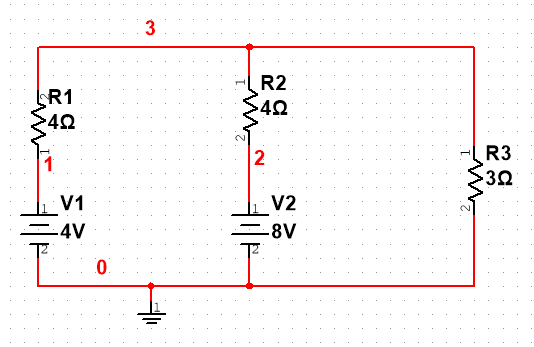
\includegraphics[width=0.6\textwidth]{A.png}
\caption{仿真电路1}
\end{figure}
\begin{figure}[H]
\centering

\includegraphics[width=0.75\textwidth]{B.png}
\caption{灵敏度分析}
\end{figure}

由仿真电路的灵敏度分析结果可见,仿真结果和理论推算符合地很好。
\subsection{结合仿真电路的讨论}
\textbf{1.若 R1, R2, R3 的阻值偏差是相互独立的, 且最大偏差均为其阻值的10\%,US1, US2 是精确不变的。U (a) 的偏差不能超过其工作点的10\%,分别用绝对灵敏度和相对灵敏度讨论能否确保电路正常工作。}

首先从绝对灵敏度角度分析:

代入对应的值,求得$\Delta U(a)_{max}=\Delta R_1\frac{\partial U(a)}{\partial R_1}+\Delta R_2\frac{\partial U(a)}{\partial R_2}+\Delta R_3\frac{\partial U(a)}{\partial R_3}=0.4\times\frac{-4\times3^2\times8+4^2\times3\times4+4\times3^2\times4}{(4\times4+4\times3+4\times3)^2}+0.4\times\frac{-4\times3^2\times4+4^2\times3\times8+4\times3^2\times8}{(4\times4+4\times3+4\times3)^2}+0.3\times\frac{4\times4^2\times4+4^2\times4\times8}{(4\times4+4\times3+4\times3)^2}=0.288$V,$\frac{\Delta U(a)_{max}}{U(a)}=\frac{0.336}{3.6}=8\%<10\%$,故而可以保证电路正常工作。

再从相对灵敏度角度分析:

代入对应的值,求得$\frac{dU(a)}{U(a)}=-\frac{4\times(4\times3^2\times8-4^2\times3\times4-4\times3^2\times4)}{(4\times4+4\times3+3\times4)\times(4\times3\times4+4\times3\times8)}\times0.1-\frac{4\times(4\times3^2\times4-4^2\times3\times8-4\times3^2\times8)}{(4\times4+4\times3+3\times4)\times(4\times3\times4+4\times3\times8)}\times0.1+\frac{3\times(4\times4^2\times4+4^2\times4\times8))}{(4\times4+4\times3+3\times4)\times(4\times3\times4+4\times3\times8)}\times0.1=8\%<10\%$,所以可以保证电路正常工作。


\textbf{2.将上述的节点电压最大偏差所对应的电阻值代入公式中,所得到的节点电压和上题中得到的有最大偏差的节点电压的差别有多大?为什么会有这样的差别?}

原本节点电压大小为$U(a)=\frac{4\times3\times4+4\times3\times8}{4\times4+4\times3+4\times3}=3.6$V,由上一题结果可得,$R_1'=3.6\Omega$,$R_2'=3.6\Omega$,$R_3'=3.3\Omega$,由公式(1)可得,$U'(a)=\frac{3.6\times3.3\times4+3.6\times3.3\times8}{3.6\times3.6+3.6\times3.3+3.6\times3.3} \approx3.88235$V,而由上一题结果,所得节点电压应为$U(a)_{expected}=108\%\times U(a)=3.888$V,差别约为0.00565V。

存在该差别的原因是,绝对灵敏度反映的是$R_1$,$R_2$,$R_3$在极小的变动范围内对U(a)产生的影响,通过该影响进行评估,而$10\%$的变动范围比较大,较为明显的差别就产生了。而且可以推知,电阻的变化范围越大,绝对灵敏度所反映的阻值变化对U(a)的影响就越会失真,越容易产生误差,因而灵敏度只可用于较小变动的影响预估,很多时候仍然需要尽可能计算出精确结果,避免利用灵敏度预估结果而产生的差别。
\section{第二题:用运算放大器实现跟随器}
本题仿真电路如下图
\subsection{仿真电路}
\begin{figure}[H]
\centering
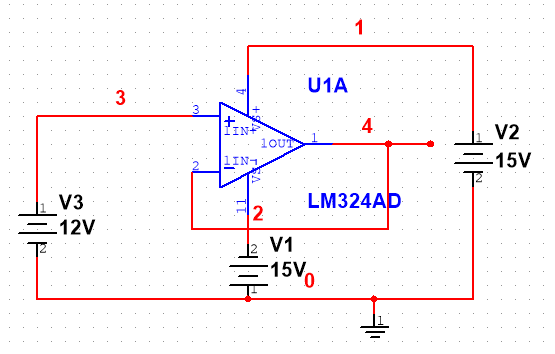
\includegraphics[width=0.95\textwidth]{C.png}
\caption{仿真电路2}
\end{figure}
\subsection{利用仿真电路得到的图表}
用参数扫描工具,测量输入信号从0V变化至20V时的输出电压,得到下图:
\begin{figure}[H]
\centering
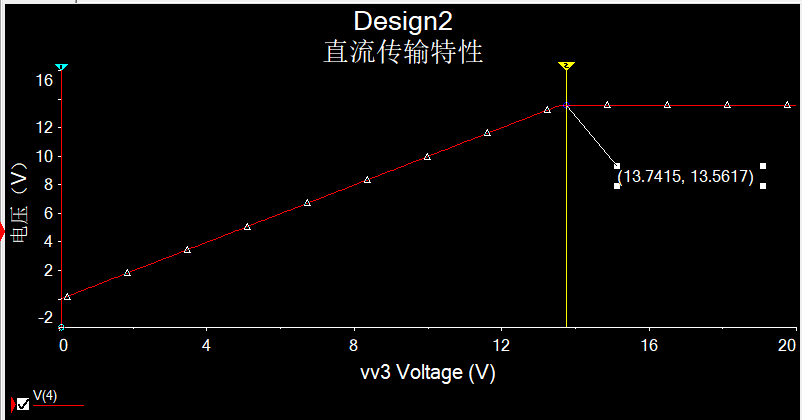
\includegraphics[width=0.8\textwidth]{D.png}
\caption{输出电压随输入电压的变化}
\end{figure}
可以看出,转折点处坐标约为(13.7415V,13.5617V),即输入电压超过13.7V后,输出电压达到饱和电压,约为13.5617V。
\section{第三题:用运算放大器实现3x+2y-0.5z的信号运算功能}
\subsection{电路原理图及分析}
电路原理图如下
\begin{figure}[H]
\centering
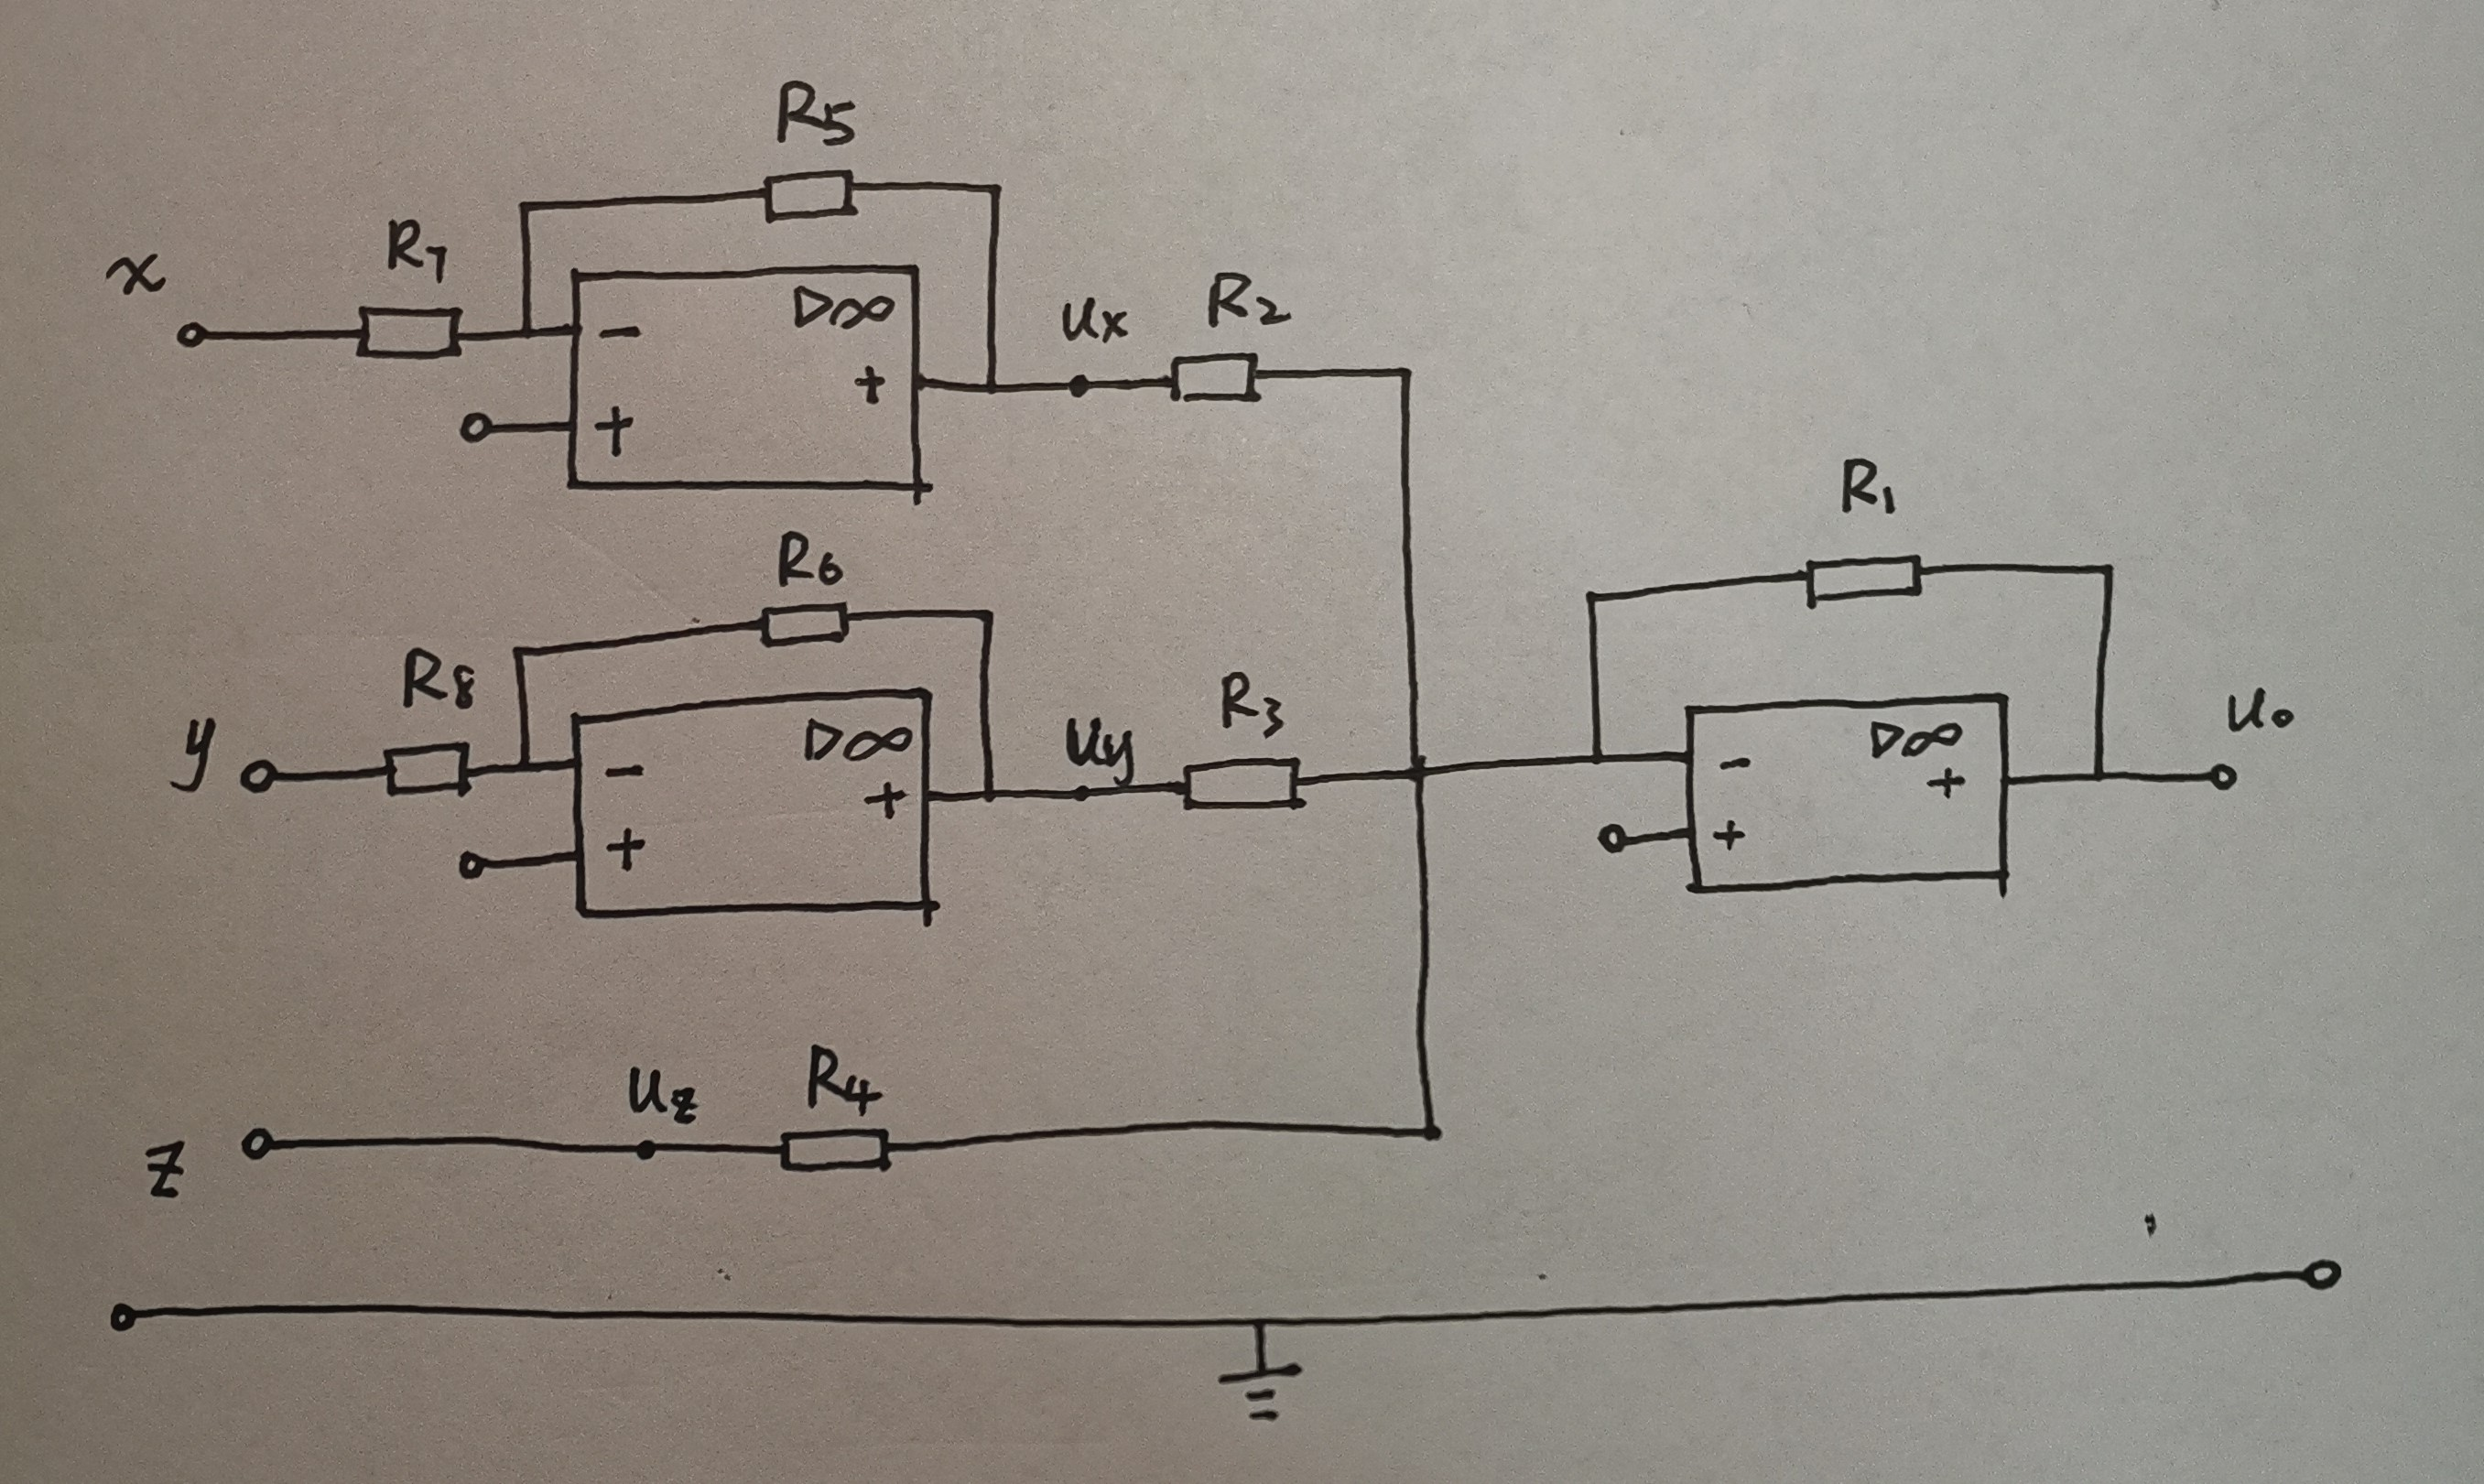
\includegraphics[width=0.95\textwidth]{F.jpg}
\caption{手绘电路原理图}
\end{figure}
此电路中的电阻阻值满足下列条件:
\begin{itemize}
\item $R_1=3R_2=2R_3=0.5R_4=6R_0$
\item $R_5=R_7$
\item $R_6=R_8$
\end{itemize}

此电路有三个输入端,对应图中和题目中的x、y、z,输出为$u_0$,采用了三个运算放大器,首先看最右侧的放大器,可看出其为加权加法器,即$u_0=-(\frac{R_1}{R_2}u_x+\frac{R_1}{R_3}u_y+\frac{R_1}{R_4}u_z)=-(3u_x+2u_y+0.5u_z)$,而左侧两个运算放大器则为反相比例放大器,即使$u_x=-\frac{R_5}{R_7}x=-x$,$u_y=-\frac{R_6}{R_8}y=-y$,而$u_z=z$,所以有$u_0=3x+2y-0.5z$。
\subsection{仿真电路}
仿真电路如下图
\begin{figure}[H]
\centering
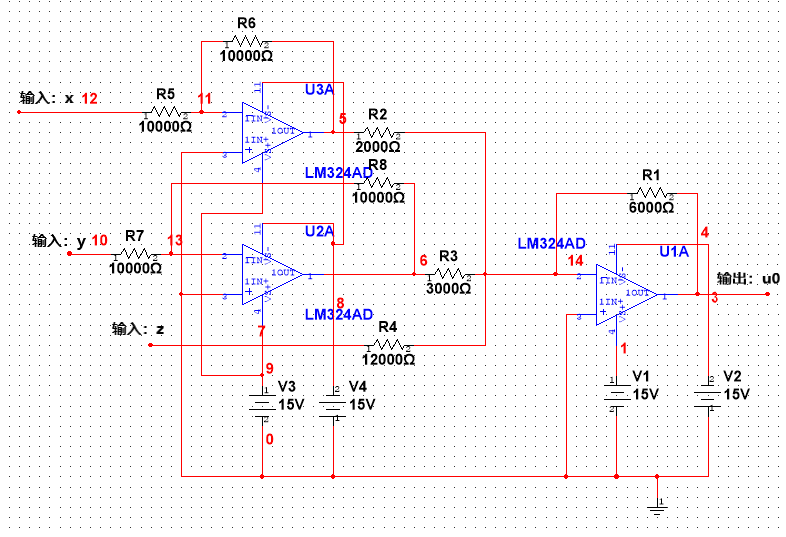
\includegraphics[width=0.95\textwidth]{E.png}
\caption{仿真电路3}
\end{figure}
\subsection{利用仿真电路进行模拟}
利用该仿真电路进行模拟,得到的数据见下表
\begin{table}[H]
    \centering
    \begin{tabular}{|l|l|l|l|l|l|l|l|l|l|l|l|l|}
    \hline
\multirow{3}{*}{ }
&\multicolumn{3}{|c|}{1} &\multicolumn{3}{|c|}{2} &\multicolumn{3}{|c|}{3} &\multicolumn{3}{|c|}{4}  \\ \cline{2-13}
         & x & y & z & x & y & z & x & y & z & x & y & z \\ \cline{2-13}
         & 1 & 1 & 1 & 1 & 3 & 2 & -2 & 2 & 0 & 3 & 3 & 2 \\ \hline
        理论输出(V) &\multicolumn{3}{|c|}{4.5}&\multicolumn{3}{|c|}{8}&\multicolumn{3}{|c|}{-2}&\multicolumn{3}{|c|}{14} \\ \hline
        仿真输出(V) &\multicolumn{3}{|c|}{4.502}&\multicolumn{3}{|c|}{8.002}&\multicolumn{3}{|c|}{-1.998}&\multicolumn{3}{|c|}{13.56} \\ \hline
    \end{tabular}
\end{table}

模拟输出中,前三个输出都正常,而最后一个输出出现异常,理论上应接近14,而输出为13.56,结合第二题可知,13.56V为所用运放的饱和电压,即最大输出只能为13.56。要解决该问题,可以将电路原理图中最右侧的运放替换为两个运放(左侧的两个运放可以删减为一个运放,使得总运放数不超过三个),即在一个运放上叠加另一个运放,以运放A(接地)的输出端作为运放B的电势零点,将运放B的输出与运放A的接地端之间的电压差作为输出,则理论上可以将最大输出扩大为原来的两倍(实际上由于两个运放不一定平均分配最终输出,所以往往达不到理论最大输出),就可以保证此题中的所有输出的正确。
\begin{thebibliography}{123456} 
\bibitem{ref1} 无
\end{thebibliography}


\end{document}
